\begin{pastexam}[label={px:ncku-106-ee-ds-07}]{成大電機所 106 學年度 簡答題第 3 題}
（簡答）

\textbf{(20 pts) Threaded binary tree.}
\begin{enumerate}[label=\alph*.]
\item \textbf{(2 pts)} How many threads are there in a threaded binary tree which contains n nodes?
\item \textbf{(5 pts)} Obtain the binary tree whose preorder traversal is ABCEDF and inorder traversal is CBDEAF.
\item \textbf{(3 pts)} Show the components in the data structure of a node in a thread binary tree and explain
their purposes.
\item \textbf{(5 pts)} Show the post-threaded binary tree corresponding to the binary tree generated by b. Make
sure that the tree does not contain any dangling thread.
\item \textbf{(5 pts)} Show the data after calling the function \textbf{OPT} if current node points to the node B
in the tree.
\begin{minted}[fontsize=\small]{cpp}
T* ThreadInorderIterator:: OPT() {
  ThreadNode <T> *temp = currentNode->rightChild;
  if (!currentNode->rightThread)
      while (!temp->leftThread) temp=temp->leftChild;
  currentNode = temp;
  if (currentNode == root) return 0;
  else return &currentNode->data;
}
\end{minted}
\end{enumerate}
\end{pastexam}

\begin{pastsoln}
答案：a.\ $n + 1$ 條；b.\ 根 $A$，$A$ 的左子 $B$、右子 $F$，$B$ 的左子 $C$、右子 $E$，$E$ 的左子 $D$；
c.\ 見下；d.\ 見下圖；e.\ $D$。

\textbf{a.} $n$ 個節點的二元樹有 $2n$ 個指標欄位，除了根以外每個節點被一個指標指著，用掉 $n - 1$ 個，空的指標
有 $2n - (n - 1) = n + 1$ 個（資結書第~7.2.2~節）。 引線二元樹把每個空指標都換成引線，所以有 $n + 1$ 條引線。
（有頭節點時，這 $n + 1$ 條裡第一個和最後一個節點的那兩條指向頭節點。）

\textbf{b.} 用前序找根、中序分左右（資結書第~7.4~節）：
\begin{itemize}
\item 前序第一個 $A$ 是根。 中序 $\underline{C\,B\,D\,E}\,A\,\underline{F}$：左子樹 $\{C, B, D, E\}$、右子樹 $\{F\}$。
\item 左子樹的前序是 $B\,C\,E\,D$，根 $B$；中序 $C\,B\,D\,E$ 分成左 $\{C\}$、右 $\{D, E\}$。
\item $\{D, E\}$ 的前序 $E\,D$，根 $E$；中序 $D\,E$，所以 $D$ 是 $E$ 的左子節點。
\end{itemize}
\begin{center}
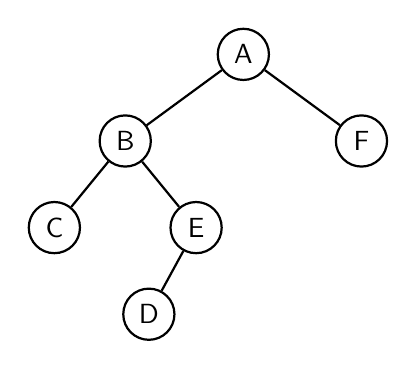
\begin{tikzpicture}[v/.style={circle,draw,thick,inner sep=0pt,minimum size=6.5mm,font=\sffamily}]
\node[v] (A) at (0,0) {A};
\node[v] (B) at (-1.5,-1.1) {B};
\node[v] (F) at (1.5,-1.1) {F};
\node[v] (C) at (-2.4,-2.2) {C};
\node[v] (E) at (-0.6,-2.2) {E};
\node[v] (D) at (-1.2,-3.3) {D};
\draw[thick] (A)--(B) (A)--(F) (B)--(C) (B)--(E) (E)--(D);
\end{tikzpicture}
\end{center}
檢查：這棵樹的前序 $A\,B\,C\,E\,D\,F$、中序 $C\,B\,D\,E\,A\,F$，和題目一樣。

\textbf{c.} 一個節點有五個欄位：
\begin{center}
\begin{tabular}{|c|c|c|c|c|}
\hline
\texttt{leftThread} & \texttt{leftChild} & \texttt{data} & \texttt{rightChild} & \texttt{rightThread} \\
\hline
\end{tabular}
\end{center}
\begin{itemize}
\item \texttt{data}：節點存的資料。
\item \texttt{leftChild}、\texttt{rightChild}：指標。 有子節點時指向子節點；沒有時改成引線，指向走訪順序裡的
前一個（左）或後一個（右）節點。
\item \texttt{leftThread}、\texttt{rightThread}：布林旗標，為真表示對應的指標是引線、不是子節點。 少了它們就分不出
一個指標是子節點還是引線，走訪時會走錯（資結書第~7.5~節的 $\mathit{lthread}$、$\mathit{rthread}$）。
\end{itemize}

\textbf{d.} 後序引線：空的左指標指向\textbf{後序}的前一個節點，空的右指標指向後序的下一個節點。 這棵樹的後序是
$C\,D\,E\,B\,F\,A$。 空指標共 $7 = n + 1$ 個：
\begin{center}
\begin{tabular}{lll}
\toprule
節點 & 左引線（後序前一個） & 右引線（後序下一個） \\
\midrule
$C$ & 頭節點（$C$ 是後序第一個） & $D$ \\
$D$ & $C$ & $E$ \\
$E$ & （有左子 $D$） & $B$ \\
$F$ & $B$ & $A$ \\
\bottomrule
\end{tabular}
\end{center}
$C$ 是後序第一個，沒有前一個節點，它的左引線如果留空就是「懸空的引線」（dangling thread）。 題目要求不能懸空，
所以加一個\textbf{頭節點}：頭節點的左指標指向根 $A$（是子節點，不是引線），$C$ 的左引線指向頭節點。 後序最後一個
是根 $A$，它的左右都有子節點，沒有右引線，不會懸空。 頭節點的右指標照慣例指向自己。

\begin{center}
\begin{tikzpicture}[v/.style={circle,draw,thick,inner sep=0pt,minimum size=6.5mm,font=\sffamily},
  t/.style={densely dashed,->,>={Stealth[length=2mm]}}]
\node[draw,thick,rectangle,minimum width=12mm,minimum height=6mm,font=\small] (H) at (0,1.3) {head};
\node[v] (A) at (0,0) {A};
\node[v] (B) at (-1.8,-1.3) {B};
\node[v] (F) at (1.8,-1.3) {F};
\node[v] (C) at (-3.0,-2.7) {C};
\node[v] (E) at (-0.6,-2.7) {E};
\node[v] (D) at (-1.4,-4.1) {D};
\draw[thick] (H)--(A) (A)--(B) (A)--(F) (B)--(C) (B)--(E) (E)--(D);
\draw[t] (C) to[out=110,in=180] (H);
\draw[t] (C) to[out=-70,in=180] (D);
\draw[t] (D) to[bend left=50] (C);
\draw[t] (D) to[out=0,in=-90] (E);
\draw[t] (E) to[out=20,in=-20] (B);
\draw[t] (F) to[out=-150,in=-30] (B);
\draw[t] (F) to[out=60,in=0] (A);
\end{tikzpicture}

實線是子節點，虛線是後序引線。
\end{center}

\textbf{e.} 這個函數就是中序引線樹的「找中序後繼」（資結書虛擬碼~7.6 的 \proc{In-Succ}），用的是\textbf{中序}引線，
所以這裡的樹是 b 小題的樹加上中序引線（和頭節點，程式裡的 \texttt{root} 就是頭節點）。 中序是
$C\,B\,D\,E\,A\,F$，$B$ 的後繼應該是 $D$。 逐行追蹤：
\begin{itemize}
\item \texttt{temp = currentNode->rightChild}：$B$ 的右指標指向 $E$。
\item $B$ 有右子節點 $E$，\texttt{rightThread} 為假，進入 \texttt{while}：$E$ 的 \texttt{leftThread} 為假（左邊有子節點
$D$），\texttt{temp} 移到 $D$；$D$ 沒有左子節點，左指標是引線，\texttt{leftThread} 為真，迴圈停。
\item \texttt{currentNode = temp}，即 $D$；$D$ 不是頭節點，回傳 \texttt{\&D->data}。
\end{itemize}
呼叫後 \texttt{currentNode} 指向 $D$，回傳的資料是 $D$。 規則就是：有右子樹時，後繼是右子樹最左邊的節點；右邊是引線
時，後繼就是引線指的節點。
\end{pastsoln}
